\documentclass[a4paper,class=article,border=5pt,tikz]{standalone}
\usetikzlibrary{intersections,angles,quotes}

\begin{document}

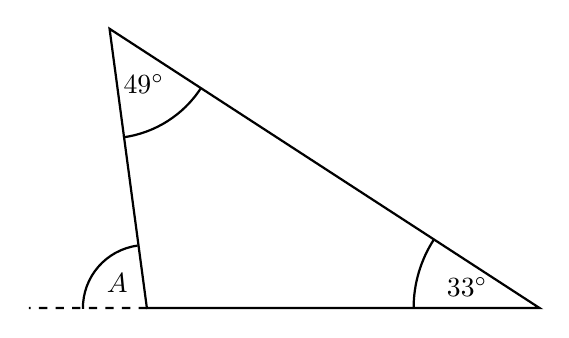
\begin{tikzpicture}[thick,scale=5,rotate=147]
\def\angleA{33} % first angle
\def\angleB{49} % second angle
\def\legAB{1}   % connecting leg
\coordinate (A) at (0,0);
\path[name path=line 1] (A) --++ (\angleA:\legAB) coordinate (C);
\path[name path=line 2] (A) --++ (0:2\legAB);
\path[name path=line 3] (C) --++ (-\angleB:2\legAB);
\path [name intersections={of=line 2 and line 3,by=B}];
\pgfresetboundingbox
\draw (A) --(B) --(C) -- cycle;
\draw pic ["$33^{\circ}$",draw,thick,angle radius=1.6cm] {angle = B--A--C};
\draw pic ["$49^{\circ}$",draw,thick,angle radius=1.4cm] {angle = C--B--A};
\draw [dashed] (C) --++ (33:0.3);
\coordinate (D) at (15,10);
\draw pic ["$A$",draw,thick,angle radius=0.8cm] {angle = B--C--D};
\end{tikzpicture}
\end{document}

